%%%%%%%%%%%%%%%%%%%%%%%%%%%%%%%%%%%%%%%%%
% University Assignment Title Page 
% LaTeX Template
% Version 1.0 (27/12/12)
%
% This template has been downloaded from:
% http://www.LaTeXTemplates.com
%
% Original author:
% WikiBooks (http://en.wikibooks.org/wiki/LaTeX/Title_Creation)
%
% License:
% CC BY-NC-SA 3.0 (http://creativecommons.org/licenses/by-nc-sa/3.0/)
% 
% Instructions for using this template:
% This title page is capable of being compiled as is. This is not useful for 
% including it in another document. To do this, you have two options: 
%
% 1) Copy/paste everything between \begin{document} and \end{document} 
% starting at \begin{titlepage} and paste this into another LaTeX file where you 
% want your title page.
% OR
% 2) Remove everything outside the \begin{titlepage} and \end{titlepage} and 
% move this file to the same directory as the LaTeX file you wish to add it to. 
% Then add %%%%%%%%%%%%%%%%%%%%%%%%%%%%%%%%%%%%%%%%%
% University Assignment Title Page 
% LaTeX Template
% Version 1.0 (27/12/12)
%
% This template has been downloaded from:
% http://www.LaTeXTemplates.com
%
% Original author:
% WikiBooks (http://en.wikibooks.org/wiki/LaTeX/Title_Creation)
%
% License:
% CC BY-NC-SA 3.0 (http://creativecommons.org/licenses/by-nc-sa/3.0/)
% 
% Instructions for using this template:
% This title page is capable of being compiled as is. This is not useful for 
% including it in another document. To do this, you have two options: 
%
% 1) Copy/paste everything between \begin{document} and \end{document} 
% starting at \begin{titlepage} and paste this into another LaTeX file where you 
% want your title page.
% OR
% 2) Remove everything outside the \begin{titlepage} and \end{titlepage} and 
% move this file to the same directory as the LaTeX file you wish to add it to. 
% Then add %%%%%%%%%%%%%%%%%%%%%%%%%%%%%%%%%%%%%%%%%
% University Assignment Title Page 
% LaTeX Template
% Version 1.0 (27/12/12)
%
% This template has been downloaded from:
% http://www.LaTeXTemplates.com
%
% Original author:
% WikiBooks (http://en.wikibooks.org/wiki/LaTeX/Title_Creation)
%
% License:
% CC BY-NC-SA 3.0 (http://creativecommons.org/licenses/by-nc-sa/3.0/)
% 
% Instructions for using this template:
% This title page is capable of being compiled as is. This is not useful for 
% including it in another document. To do this, you have two options: 
%
% 1) Copy/paste everything between \begin{document} and \end{document} 
% starting at \begin{titlepage} and paste this into another LaTeX file where you 
% want your title page.
% OR
% 2) Remove everything outside the \begin{titlepage} and \end{titlepage} and 
% move this file to the same directory as the LaTeX file you wish to add it to. 
% Then add %%%%%%%%%%%%%%%%%%%%%%%%%%%%%%%%%%%%%%%%%
% University Assignment Title Page 
% LaTeX Template
% Version 1.0 (27/12/12)
%
% This template has been downloaded from:
% http://www.LaTeXTemplates.com
%
% Original author:
% WikiBooks (http://en.wikibooks.org/wiki/LaTeX/Title_Creation)
%
% License:
% CC BY-NC-SA 3.0 (http://creativecommons.org/licenses/by-nc-sa/3.0/)
% 
% Instructions for using this template:
% This title page is capable of being compiled as is. This is not useful for 
% including it in another document. To do this, you have two options: 
%
% 1) Copy/paste everything between \begin{document} and \end{document} 
% starting at \begin{titlepage} and paste this into another LaTeX file where you 
% want your title page.
% OR
% 2) Remove everything outside the \begin{titlepage} and \end{titlepage} and 
% move this file to the same directory as the LaTeX file you wish to add it to. 
% Then add \input{./title_page_1.tex} to your LaTeX file where you want your
% title page.
%
%%%%%%%%%%%%%%%%%%%%%%%%%%%%%%%%%%%%%%%%%

%----------------------------------------------------------------------------------------
%	PACKAGES AND OTHER DOCUMENT CONFIGURATIONS
%----------------------------------------------------------------------------------------

\documentclass[12pt, showidx]{article}

\usepackage[utf8]{inputenc}
\usepackage[T1]{fontenc}
\usepackage{lmodern}
\usepackage{parselines}
\usepackage[portuguese]{babel}
\usepackage{graphicx}
\usepackage{imakeidx}
\usepackage[document]{ragged2e}

\graphicspath{ {images/} }

\makeindex[title = Palavras Chave]

\begin{document}

\begin{titlepage}

\newcommand{\HRule}{\rule{\linewidth}{1mm}} % Defines a new command for the horizontal lines, change thickness here

\center % Center everything on the page
 
%----------------------------------------------------------------------------------------
%	HEADING SECTIONS
%----------------------------------------------------------------------------------------


\includegraphics{feup.jpg}

\textsc{\large Inteligência Artificial}\\[0.5cm] % Major heading such as course name
\textsc{\large 3º ano do Mestrado Integrado em Engenharia Informática e Computação}\\[0.5cm] % Minor heading such as course title

%----------------------------------------------------------------------------------------
%	TITLE SECTION
%----------------------------------------------------------------------------------------

\HRule \\[0.4cm]
{ \huge \bfseries Otimização da gestão de projetos}\\[0.2cm] % Title of your document
\HRule \\[1cm]
 
%----------------------------------------------------------------------------------------
%	AUTHOR SECTION
%----------------------------------------------------------------------------------------


% If you don't want a supervisor, uncomment the two lines below and remove the section above
\Large \emph{Authors:}\\
Duarte \textsc{Pinto}\\[0cm] - up201304777 
- up201304777@fe.up.pt\\[0cm]
Filipa \textsc{Ramos}\\[0cm] - up201305378
- up201305378@fe.up.pt\\[0cm] 
Gustavo \textsc{Silva}\\[0cm] - up201304143
- up201304143@fe.up.pt\\[1cm] % Your name

%----------------------------------------------------------------------------------------
%	DATE SECTION
%----------------------------------------------------------------------------------------

{\large \today}\\[0cm] % Date, change the \today to a set date if you want to be precise

%----------------------------------------------------------------------------------------
%	TABLE OF CONTENTS & LISTS OF FIGURES AND TABLES
%----------------------------------------------------------------------------------------

\tableofcontents

%----------------------------------------------------------------------------------------
%	INTRODUÇÃO
%----------------------------------------------------------------------------------------

\section{Introdução} 

\justify\normalsize
No âmbito da unidade curricular de Inteligência Artificial pretende-se desenvolver um programa que, com base em algoritmos genéticos e arrefecimento simulado, faça a gestão de um projeto balançando os elementos participantes e as tarefas a realizar do mesmo. O sistema é composto por um conjunto de tarefas que pertencem ao projeto em análise. Cada tarefa tem uma competência indispensável ao seu cumprimento e uma duração. Cada elemento tem um conjunto de competências sendo que o mesmo tem um nível de capacidade para cumprir cada uma. A gestão a ser realizada tem em vista minimizar o tempo ocupado para satisfazer todas as tarefas do projeto usando a melhor combinação de elementos para cada tarefa. Será feita uma análise comparativa entre o desempenho das solução encontradas com algoritmos genéticos e arrefecimento simulado. 

Os objetivos principais do projeto passam pela exploração da implementação prática dos algoritmos genéticos e do algoritmo de arrefecimento simulado. Através dos dados obtidos, visa-se também realizar uma comparação da solução encontrada com ambos os algoritmos. Este processo irá fomentar o conhecimento adquirido, evidenciando as vantagens principais de cada algoritmo e as suas dicotomias principais.  

Espera-se que surjam dificuldades na implementação prática dos algoritmos estudados teoricamente, principalmente na construção dos cromossomas pois existem dúvidas em relação à sua influência na eficiência da solução encontrada. Para além disto, a melhor adaptação da função de avaliação ao problema por forma a obter os melhores resultados revela-se um processo tumultuoso. Os membros decidiram optar por otimizar o tempo utilizado a concluir todas as tarefas do projeto em estudo. Desta forma, a melhor solução será a que implicará um menor tempo de conclusão do projeto em questão.

%----------------------------------------------------------------------------------------

\newpage % Start the article content on the second page, remove this if you have a longer abstract that goes onto the second page

%----------------------------------------------------------------------------------------
%	ESPECIFICAÇÃO
%----------------------------------------------------------------------------------------

\section{Especificação}

\subsection{Problematização}
\justify\normalsize
O sistema tem por objetivo otimizar a atribuição de membros por tarefas num dado projeto. Os dados do mesmo são introduzidos por input através de um ficheiro.

Um projeto em análise caracteriza-se por um conjunto de tarefas (\index{Task} Task) a cumprir, tendo estas um nome (por motivos de identificação) e uma duração. Existe ainda um conjunto de elementos (\index{Element} Element) que podem ser atribuídos a essas mesmas tarefas. Um elemento é identificado por um nome e tem uma lista de competências (\index{Skill} Skill) avaliadas em função da sua capacidade. Por exemplo, o elemento "joão" tem competências na área da informática a um nível 6 e na área da economia com nível 10.

\subsection{Aquitetura}
\justify\normalsize
O projeto foi dividido em três "packages" principais que representam os três níveis mais importantes. Um dos packages diz respeito às classes que guardam informação sobre as tarefas, os elementos e as competências. Os outros dois dizem respeito à implementação do algoritmo genético ou do arrefecimento simulado.

A arquitetura pensada para o projeto passa pela implementação de três classes principais que interagem entre si próprias. A classe "Task" representa uma tarefa e guarda a sua duração. Um elemento é representado pela classe "Element" que mantém a identificação do mesmo. A classe "Skill" corresponde a uma competência. Estas ligam-se entre si por forma a que um elemento tenha vários skills e um skill tenha várias tarefas tal como é visível na figura \ref{fig:uml}.

\begin{figure}[h]
  \centering
    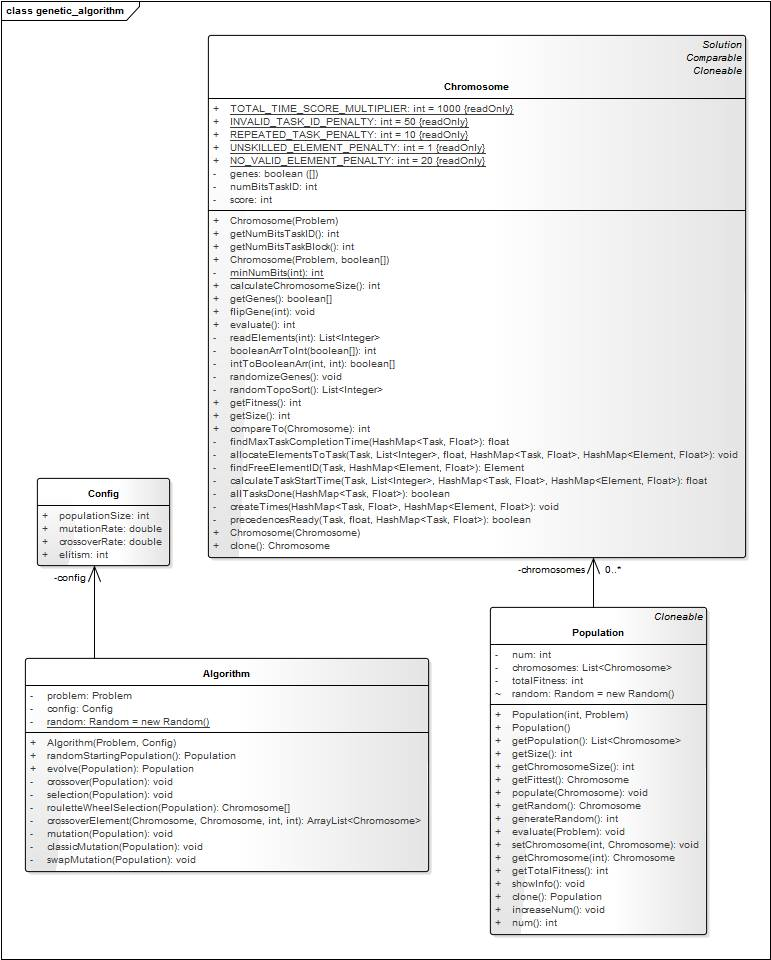
\includegraphics[width=10cm, height = 10cm]{uml.jpg}
  \caption{Diagrama de classes UML}
  \label{fig:uml}
\end{figure}

\subsection{Fases}
\justify\normalsize 
O projeto será dividido em fases de trabalho. A inicial passa pelo desenvolvimento da arquitetura explicitada em cima. Seguidamente, proceder-se-á implementação dos \index{Algortimos Genéticos} algoritmos genéticos. Finalmente, será desenvolvido o arrefecimento simulado. As fases abordadas até ao presente relatório foram as duas primeiras. A arquitetura explicitada pelo diagrama de classes uml já foi implementada e a obtenção de solução por algoritmos genéticos encontra-se numa fase avançada.

\subsection{Algoritmos Genéticos}
\justify\normalsize
Explicar o algoritmo usado:
	- estrutura do cromossoma
	- função de avaliação
	- seleção
	- cruzamento
	- mutações

\subsection{Arrefecimento Simulado}
\justify\normalsize
Explicar o algoritmo usado.

\section{Trabalho Realizado}
\justify\normalsize
Incluir trechos do código já implementado.

\section{Testes}
\justify\normalsize
Explicar os testes planeados.

\section{Conclusões}
\justify\normalsize
Conclusões retiradas.

\printindex

\end{titlepage}
\end{document} to your LaTeX file where you want your
% title page.
%
%%%%%%%%%%%%%%%%%%%%%%%%%%%%%%%%%%%%%%%%%

%----------------------------------------------------------------------------------------
%	PACKAGES AND OTHER DOCUMENT CONFIGURATIONS
%----------------------------------------------------------------------------------------

\documentclass[12pt, showidx]{article}

\usepackage[utf8]{inputenc}
\usepackage[T1]{fontenc}
\usepackage{lmodern}
\usepackage{parselines}
\usepackage[portuguese]{babel}
\usepackage{graphicx}
\usepackage{imakeidx}
\usepackage[document]{ragged2e}

\graphicspath{ {images/} }

\makeindex[title = Palavras Chave]

\begin{document}

\begin{titlepage}

\newcommand{\HRule}{\rule{\linewidth}{1mm}} % Defines a new command for the horizontal lines, change thickness here

\center % Center everything on the page
 
%----------------------------------------------------------------------------------------
%	HEADING SECTIONS
%----------------------------------------------------------------------------------------


\includegraphics{feup.jpg}

\textsc{\large Inteligência Artificial}\\[0.5cm] % Major heading such as course name
\textsc{\large 3º ano do Mestrado Integrado em Engenharia Informática e Computação}\\[0.5cm] % Minor heading such as course title

%----------------------------------------------------------------------------------------
%	TITLE SECTION
%----------------------------------------------------------------------------------------

\HRule \\[0.4cm]
{ \huge \bfseries Otimização da gestão de projetos}\\[0.2cm] % Title of your document
\HRule \\[1cm]
 
%----------------------------------------------------------------------------------------
%	AUTHOR SECTION
%----------------------------------------------------------------------------------------


% If you don't want a supervisor, uncomment the two lines below and remove the section above
\Large \emph{Authors:}\\
Duarte \textsc{Pinto}\\[0cm] - up201304777 
- up201304777@fe.up.pt\\[0cm]
Filipa \textsc{Ramos}\\[0cm] - up201305378
- up201305378@fe.up.pt\\[0cm] 
Gustavo \textsc{Silva}\\[0cm] - up201304143
- up201304143@fe.up.pt\\[1cm] % Your name

%----------------------------------------------------------------------------------------
%	DATE SECTION
%----------------------------------------------------------------------------------------

{\large \today}\\[0cm] % Date, change the \today to a set date if you want to be precise

%----------------------------------------------------------------------------------------
%	TABLE OF CONTENTS & LISTS OF FIGURES AND TABLES
%----------------------------------------------------------------------------------------

\tableofcontents

%----------------------------------------------------------------------------------------
%	INTRODUÇÃO
%----------------------------------------------------------------------------------------

\section{Introdução} 

\justify\normalsize
No âmbito da unidade curricular de Inteligência Artificial pretende-se desenvolver um programa que, com base em algoritmos genéticos e arrefecimento simulado, faça a gestão de um projeto balançando os elementos participantes e as tarefas a realizar do mesmo. O sistema é composto por um conjunto de tarefas que pertencem ao projeto em análise. Cada tarefa tem uma competência indispensável ao seu cumprimento e uma duração. Cada elemento tem um conjunto de competências sendo que o mesmo tem um nível de capacidade para cumprir cada uma. A gestão a ser realizada tem em vista minimizar o tempo ocupado para satisfazer todas as tarefas do projeto usando a melhor combinação de elementos para cada tarefa. Será feita uma análise comparativa entre o desempenho das solução encontradas com algoritmos genéticos e arrefecimento simulado. 

Os objetivos principais do projeto passam pela exploração da implementação prática dos algoritmos genéticos e do algoritmo de arrefecimento simulado. Através dos dados obtidos, visa-se também realizar uma comparação da solução encontrada com ambos os algoritmos. Este processo irá fomentar o conhecimento adquirido, evidenciando as vantagens principais de cada algoritmo e as suas dicotomias principais.  

Espera-se que surjam dificuldades na implementação prática dos algoritmos estudados teoricamente, principalmente na construção dos cromossomas pois existem dúvidas em relação à sua influência na eficiência da solução encontrada. Para além disto, a melhor adaptação da função de avaliação ao problema por forma a obter os melhores resultados revela-se um processo tumultuoso. Os membros decidiram optar por otimizar o tempo utilizado a concluir todas as tarefas do projeto em estudo. Desta forma, a melhor solução será a que implicará um menor tempo de conclusão do projeto em questão.

%----------------------------------------------------------------------------------------

\newpage % Start the article content on the second page, remove this if you have a longer abstract that goes onto the second page

%----------------------------------------------------------------------------------------
%	ESPECIFICAÇÃO
%----------------------------------------------------------------------------------------

\section{Especificação}

\subsection{Problematização}
\justify\normalsize
O sistema tem por objetivo otimizar a atribuição de membros por tarefas num dado projeto. Os dados do mesmo são introduzidos por input através de um ficheiro.

Um projeto em análise caracteriza-se por um conjunto de tarefas (\index{Task} Task) a cumprir, tendo estas um nome (por motivos de identificação) e uma duração. Existe ainda um conjunto de elementos (\index{Element} Element) que podem ser atribuídos a essas mesmas tarefas. Um elemento é identificado por um nome e tem uma lista de competências (\index{Skill} Skill) avaliadas em função da sua capacidade. Por exemplo, o elemento "joão" tem competências na área da informática a um nível 6 e na área da economia com nível 10.

\subsection{Aquitetura}
\justify\normalsize
O projeto foi dividido em três "packages" principais que representam os três níveis mais importantes. Um dos packages diz respeito às classes que guardam informação sobre as tarefas, os elementos e as competências. Os outros dois dizem respeito à implementação do algoritmo genético ou do arrefecimento simulado.

A arquitetura pensada para o projeto passa pela implementação de três classes principais que interagem entre si próprias. A classe "Task" representa uma tarefa e guarda a sua duração. Um elemento é representado pela classe "Element" que mantém a identificação do mesmo. A classe "Skill" corresponde a uma competência. Estas ligam-se entre si por forma a que um elemento tenha vários skills e um skill tenha várias tarefas tal como é visível na figura \ref{fig:uml}.

\begin{figure}[h]
  \centering
    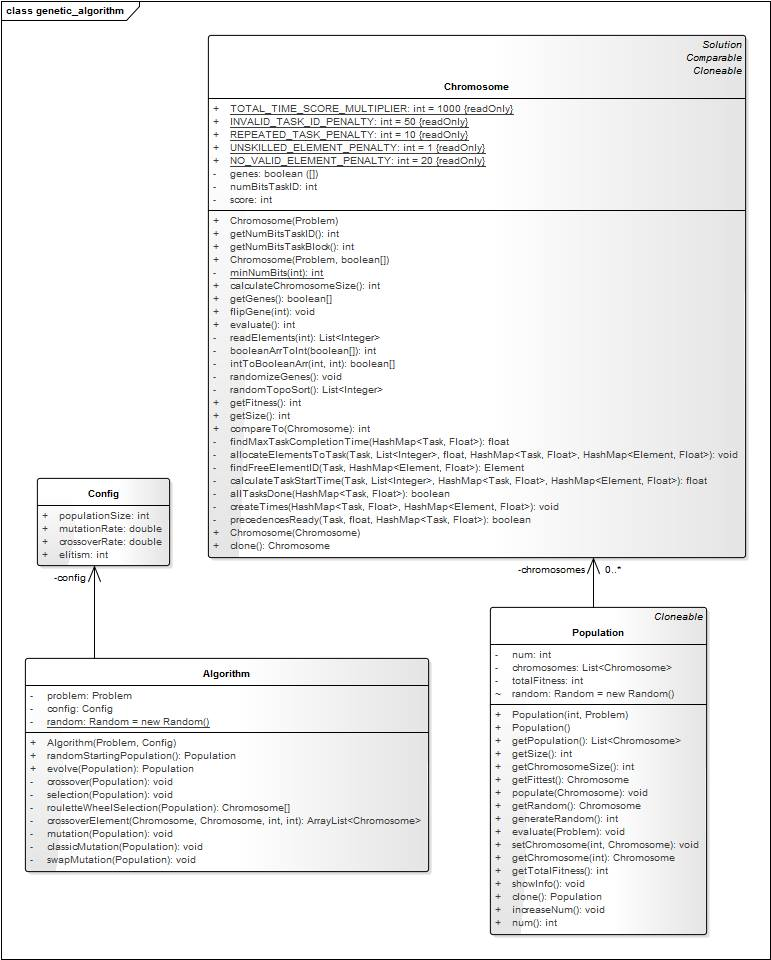
\includegraphics[width=10cm, height = 10cm]{uml.jpg}
  \caption{Diagrama de classes UML}
  \label{fig:uml}
\end{figure}

\subsection{Fases}
\justify\normalsize 
O projeto será dividido em fases de trabalho. A inicial passa pelo desenvolvimento da arquitetura explicitada em cima. Seguidamente, proceder-se-á implementação dos \index{Algortimos Genéticos} algoritmos genéticos. Finalmente, será desenvolvido o arrefecimento simulado. As fases abordadas até ao presente relatório foram as duas primeiras. A arquitetura explicitada pelo diagrama de classes uml já foi implementada e a obtenção de solução por algoritmos genéticos encontra-se numa fase avançada.

\subsection{Algoritmos Genéticos}
\justify\normalsize
Explicar o algoritmo usado:
	- estrutura do cromossoma
	- função de avaliação
	- seleção
	- cruzamento
	- mutações

\subsection{Arrefecimento Simulado}
\justify\normalsize
Explicar o algoritmo usado.

\section{Trabalho Realizado}
\justify\normalsize
Incluir trechos do código já implementado.

\section{Testes}
\justify\normalsize
Explicar os testes planeados.

\section{Conclusões}
\justify\normalsize
Conclusões retiradas.

\printindex

\end{titlepage}
\end{document} to your LaTeX file where you want your
% title page.
%
%%%%%%%%%%%%%%%%%%%%%%%%%%%%%%%%%%%%%%%%%

%----------------------------------------------------------------------------------------
%	PACKAGES AND OTHER DOCUMENT CONFIGURATIONS
%----------------------------------------------------------------------------------------

\documentclass[12pt, showidx]{article}

\usepackage[utf8]{inputenc}
\usepackage[T1]{fontenc}
\usepackage{lmodern}
\usepackage{parselines}
\usepackage[portuguese]{babel}
\usepackage{graphicx}
\usepackage{imakeidx}
\usepackage[document]{ragged2e}

\graphicspath{ {images/} }

\makeindex[title = Palavras Chave]

\begin{document}

\begin{titlepage}

\newcommand{\HRule}{\rule{\linewidth}{1mm}} % Defines a new command for the horizontal lines, change thickness here

\center % Center everything on the page
 
%----------------------------------------------------------------------------------------
%	HEADING SECTIONS
%----------------------------------------------------------------------------------------


\includegraphics{feup.jpg}

\textsc{\large Inteligência Artificial}\\[0.5cm] % Major heading such as course name
\textsc{\large 3º ano do Mestrado Integrado em Engenharia Informática e Computação}\\[0.5cm] % Minor heading such as course title

%----------------------------------------------------------------------------------------
%	TITLE SECTION
%----------------------------------------------------------------------------------------

\HRule \\[0.4cm]
{ \huge \bfseries Otimização da gestão de projetos}\\[0.2cm] % Title of your document
\HRule \\[1cm]
 
%----------------------------------------------------------------------------------------
%	AUTHOR SECTION
%----------------------------------------------------------------------------------------


% If you don't want a supervisor, uncomment the two lines below and remove the section above
\Large \emph{Authors:}\\
Duarte \textsc{Pinto}\\[0cm] - up201304777 
- up201304777@fe.up.pt\\[0cm]
Filipa \textsc{Ramos}\\[0cm] - up201305378
- up201305378@fe.up.pt\\[0cm] 
Gustavo \textsc{Silva}\\[0cm] - up201304143
- up201304143@fe.up.pt\\[1cm] % Your name

%----------------------------------------------------------------------------------------
%	DATE SECTION
%----------------------------------------------------------------------------------------

{\large \today}\\[0cm] % Date, change the \today to a set date if you want to be precise

%----------------------------------------------------------------------------------------
%	TABLE OF CONTENTS & LISTS OF FIGURES AND TABLES
%----------------------------------------------------------------------------------------

\tableofcontents

%----------------------------------------------------------------------------------------
%	INTRODUÇÃO
%----------------------------------------------------------------------------------------

\section{Introdução} 

\justify\normalsize
No âmbito da unidade curricular de Inteligência Artificial pretende-se desenvolver um programa que, com base em algoritmos genéticos e arrefecimento simulado, faça a gestão de um projeto balançando os elementos participantes e as tarefas a realizar do mesmo. O sistema é composto por um conjunto de tarefas que pertencem ao projeto em análise. Cada tarefa tem uma competência indispensável ao seu cumprimento e uma duração. Cada elemento tem um conjunto de competências sendo que o mesmo tem um nível de capacidade para cumprir cada uma. A gestão a ser realizada tem em vista minimizar o tempo ocupado para satisfazer todas as tarefas do projeto usando a melhor combinação de elementos para cada tarefa. Será feita uma análise comparativa entre o desempenho das solução encontradas com algoritmos genéticos e arrefecimento simulado. 

Os objetivos principais do projeto passam pela exploração da implementação prática dos algoritmos genéticos e do algoritmo de arrefecimento simulado. Através dos dados obtidos, visa-se também realizar uma comparação da solução encontrada com ambos os algoritmos. Este processo irá fomentar o conhecimento adquirido, evidenciando as vantagens principais de cada algoritmo e as suas dicotomias principais.  

Espera-se que surjam dificuldades na implementação prática dos algoritmos estudados teoricamente, principalmente na construção dos cromossomas pois existem dúvidas em relação à sua influência na eficiência da solução encontrada. Para além disto, a melhor adaptação da função de avaliação ao problema por forma a obter os melhores resultados revela-se um processo tumultuoso. Os membros decidiram optar por otimizar o tempo utilizado a concluir todas as tarefas do projeto em estudo. Desta forma, a melhor solução será a que implicará um menor tempo de conclusão do projeto em questão.

%----------------------------------------------------------------------------------------

\newpage % Start the article content on the second page, remove this if you have a longer abstract that goes onto the second page

%----------------------------------------------------------------------------------------
%	ESPECIFICAÇÃO
%----------------------------------------------------------------------------------------

\section{Especificação}

\subsection{Problematização}
\justify\normalsize
O sistema tem por objetivo otimizar a atribuição de membros por tarefas num dado projeto. Os dados do mesmo são introduzidos por input através de um ficheiro.

Um projeto em análise caracteriza-se por um conjunto de tarefas (\index{Task} Task) a cumprir, tendo estas um nome (por motivos de identificação) e uma duração. Existe ainda um conjunto de elementos (\index{Element} Element) que podem ser atribuídos a essas mesmas tarefas. Um elemento é identificado por um nome e tem uma lista de competências (\index{Skill} Skill) avaliadas em função da sua capacidade. Por exemplo, o elemento "joão" tem competências na área da informática a um nível 6 e na área da economia com nível 10.

\subsection{Aquitetura}
\justify\normalsize
O projeto foi dividido em três "packages" principais que representam os três níveis mais importantes. Um dos packages diz respeito às classes que guardam informação sobre as tarefas, os elementos e as competências. Os outros dois dizem respeito à implementação do algoritmo genético ou do arrefecimento simulado.

A arquitetura pensada para o projeto passa pela implementação de três classes principais que interagem entre si próprias. A classe "Task" representa uma tarefa e guarda a sua duração. Um elemento é representado pela classe "Element" que mantém a identificação do mesmo. A classe "Skill" corresponde a uma competência. Estas ligam-se entre si por forma a que um elemento tenha vários skills e um skill tenha várias tarefas tal como é visível na figura \ref{fig:uml}.

\begin{figure}[h]
  \centering
    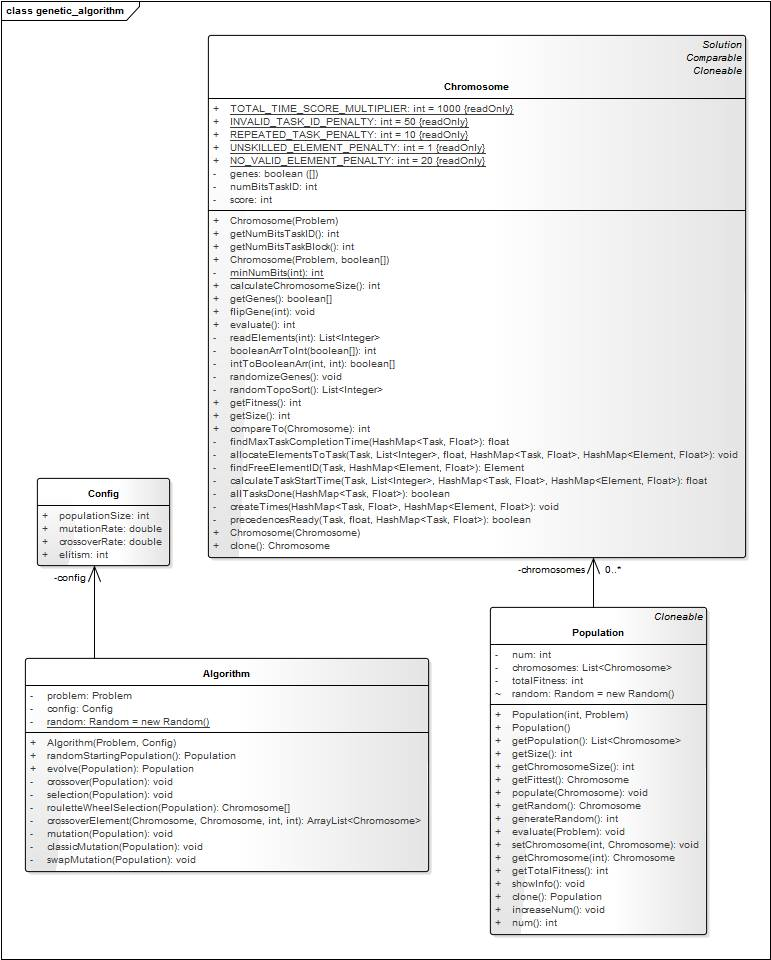
\includegraphics[width=10cm, height = 10cm]{uml.jpg}
  \caption{Diagrama de classes UML}
  \label{fig:uml}
\end{figure}

\subsection{Fases}
\justify\normalsize 
O projeto será dividido em fases de trabalho. A inicial passa pelo desenvolvimento da arquitetura explicitada em cima. Seguidamente, proceder-se-á implementação dos \index{Algortimos Genéticos} algoritmos genéticos. Finalmente, será desenvolvido o arrefecimento simulado. As fases abordadas até ao presente relatório foram as duas primeiras. A arquitetura explicitada pelo diagrama de classes uml já foi implementada e a obtenção de solução por algoritmos genéticos encontra-se numa fase avançada.

\subsection{Algoritmos Genéticos}
\justify\normalsize
Explicar o algoritmo usado:
	- estrutura do cromossoma
	- função de avaliação
	- seleção
	- cruzamento
	- mutações

\subsection{Arrefecimento Simulado}
\justify\normalsize
Explicar o algoritmo usado.

\section{Trabalho Realizado}
\justify\normalsize
Incluir trechos do código já implementado.

\section{Testes}
\justify\normalsize
Explicar os testes planeados.

\section{Conclusões}
\justify\normalsize
Conclusões retiradas.

\printindex

\end{titlepage}
\end{document} to your LaTeX file where you want your
% title page.
%
%%%%%%%%%%%%%%%%%%%%%%%%%%%%%%%%%%%%%%%%%

%----------------------------------------------------------------------------------------
%	PACKAGES AND OTHER DOCUMENT CONFIGURATIONS
%----------------------------------------------------------------------------------------

\documentclass[12pt]{article}

\usepackage[utf8]{inputenc}
\usepackage[T1]{fontenc}
\usepackage{lmodern}
\usepackage{parselines}
\usepackage[portuguese]{babel}
\usepackage{graphicx}
\usepackage[document]{ragged2e}
\usepackage{listings}
\usepackage{xcolor}
\usepackage[margin=0.8in]{geometry}		
\usepackage{amsmath}
\usepackage{hyperref}
\usepackage{url}
\usepackage{titlesec}
\usepackage{csquotes}
\usepackage{caption}
\usepackage{subcaption}
\usepackage{float}

\setcounter{secnumdepth}{4}

\titleformat{\paragraph}
{\normalfont\normalsize\bfseries}{\theparagraph}{1em}{}
\titlespacing*{\paragraph}
{0pt}{3.25ex plus 1ex minus .2ex}{1.5ex plus .2ex}

\graphicspath{ {images/} }

\colorlet{punct}{red!60!black}
\definecolor{background}{HTML}{EEEEEE}
\definecolor{delim}{RGB}{20,105,176}
\colorlet{numb}{magenta!60!black}


\lstdefinelanguage{json}{
    basicstyle=\normalfont\ttfamily,
    numbers=left,
    numberstyle=\scriptsize,
    stepnumber=1,
    numbersep=8pt,
    showstringspaces=false,
    breaklines=true,
    frame=lines,
    backgroundcolor=\color{background},
    literate=
     *{0}{{{\color{numb}0}}}{1}
      {1}{{{\color{numb}1}}}{1}
      {2}{{{\color{numb}2}}}{1}
      {3}{{{\color{numb}3}}}{1}
      {4}{{{\color{numb}4}}}{1}
      {5}{{{\color{numb}5}}}{1}
      {6}{{{\color{numb}6}}}{1}
      {7}{{{\color{numb}7}}}{1}
      {8}{{{\color{numb}8}}}{1}
      {9}{{{\color{numb}9}}}{1}
      {:}{{{\color{punct}{:}}}}{1}
      {,}{{{\color{punct}{,}}}}{1}
      {\{}{{{\color{delim}{\{}}}}{1}
      {\}}{{{\color{delim}{\}}}}}{1}
      {[}{{{\color{delim}{[}}}}{1}
      {]}{{{\color{delim}{]}}}}{1},
}

\definecolor{dkgreen}{rgb}{0,0.6,0}
\definecolor{gray}{rgb}{0.5,0.5,0.5}
\definecolor{mauve}{rgb}{0.58,0,0.82}

\lstset{frame=tb,
  language=Java,
  aboveskip=3mm,
  belowskip=3mm,
  showstringspaces=false,
  columns=flexible,
  basicstyle={\small\ttfamily},
  numbers=none,
  numberstyle=\tiny\color{gray},
  keywordstyle=\color{blue},
  commentstyle=\color{dkgreen},
  stringstyle=\color{mauve},
  breaklines=true,
  breakatwhitespace=true,
  tabsize=3
}

\begin{document}

\begin{titlepage}

\newcommand{\HRule}{\rule{\linewidth}{1mm}} % Defines a new command for the horizontal lines, change thickness here

\center % Center everything on the page
 
%----------------------------------------------------------------------------------------
%	HEADING SECTIONS
%----------------------------------------------------------------------------------------


\includegraphics{feup.jpg}

\textsc{\large Inteligência Artificial}\\[0.8cm] % Major heading such as course name
\textsc{\large 3º ano do Mestrado Integrado em Engenharia Informática e Computação}\\[0.8cm] % Minor heading such as course title

%----------------------------------------------------------------------------------------
%	TITLE SECTION
%----------------------------------------------------------------------------------------

\HRule \\[1.2cm]
{ \huge \bfseries Otimização da gestão de projetos}\\[0.6cm] % Title of your document
\HRule \\[3cm]
 
%----------------------------------------------------------------------------------------
%	AUTHOR SECTION
%----------------------------------------------------------------------------------------


% If you don't want a supervisor, uncomment the two lines below and remove the section above
\Large \emph{Authors:}\\[0.5cm] \normalsize
Duarte \textsc{Pinto}\\[0.1cm] - up201304777 
- up201304777@fe.up.pt\\[0.1cm]
Filipa \textsc{Ramos}\\[0.1cm] - up201305378
- up201305378@fe.up.pt\\[0.1cm] 
Gustavo \textsc{Silva}\\[0.1cm] - up201304143
- up201304143@fe.up.pt\\[3cm] % Your name

%----------------------------------------------------------------------------------------
%	DATE SECTION
%----------------------------------------------------------------------------------------

{\large \today}\\[0cm] % Date, change the \today to a set date if you want to be precise

%----------------------------------------------------------------------------------------
%	TABLE OF CONTENTS & LISTS OF FIGURES AND TABLES
%----------------------------------------------------------------------------------------

\tableofcontents

%----------------------------------------------------------------------------------------
%	INTRODUÇÃO
%----------------------------------------------------------------------------------------

\section{Introdução} 
\enquote{The scheduling of tasks and the allocation of resource in medium to large-scale development projects is an extremely hard problem and is one of the principal challenges of project management due to its sheer complexity.}\footnote{Carl K. Chang et al, \textit{Genetic Algorithms for Project Management}, (Holanda: Kluwer Academic Publishers, 2001)}

\justify\normalsize
No âmbito da unidade curricular de Inteligência Artificial foi desenvolvido um programa de otimização que tem por objetivo gerir projetos. Tendo por pressuposto a citação explicitada acima foi implementado um sistema para alocar membros a um projeto da maneira mais eficiente tendo em consideração a duração de cada tarefa e as competências de cada membro para cada tarefa. Pretende-se no presente documento avaliar comparativamente os resultados demonstrados por cada um dos algoritmos de otimização usados - algoritmos genéticos e arrefecimento simulado. Inicialmente será esmiuçado o problema sugerido e a perspetiva das soluções implementadas. Nesta especificação será englobada uma análise detalhada ao tema e aos cenários problemáticos que surgiram nessa mesma análise. A abordagem técnica adaptada de forma a solucionar estes obstáculos será pormenorizadamente descrita.

Um dos objetivos principais do presente documento é avaliar a resposta de ambos os algoritmos em cenários semelhantes por forma a melhor compreender a sua eficiência e as suas situações de risco. As conclusões retiradas das experiências efetuadas serão indispensáveis à exploração das possibilidades e fraquezas de cada algoritmo. Para além disto, surgem objetivos secundários tais como o aprofundamento do estudo de métodos de inteligência artificial e o estudo da aplicação prática da teoria abordada nas aulas.

%----------------------------------------------------------------------------------------

 % Start the article content on the second page, remove this if you have a longer abstract that goes onto the second page

%----------------------------------------------------------------------------------------
%	ESPECIFICAÇÃO
%----------------------------------------------------------------------------------------

\section{Especificação}

\subsection{Problematização}

\enquote{Um projeto é constituído por um conjunto de tarefas a desenvolver por um ou mais elementos. As tarefas podem ter precedências entre si e têm uma duração (pessoa/mês). Cada elemento candidato possui um conjunto de competências, que cobrem uma ou mais tarefas. É conhecido ainda o desempenho de um elemento em cada uma das suas competências.}\footnote{Enunciado do problema.}

\justify\normalsize
Como é especificado em cima o sistema tem por objetivo otimizar a atribuição de membros por tarefas num dado projeto. Os dados do mesmo são introduzidos por input através de um ficheiro no formato json no qual estão representadas as tarefas, elementos e as competências de cada um deles.

Um projeto em análise caracteriza-se por um conjunto de tarefas (Task) a cumprir, tendo estas um nome (por motivos de identificação) e uma duração. Existe ainda um conjunto de elementos (Element) que podem ser atribuídos a essas mesmas tarefas. Um elemento é identificado por um nome e tem uma lista de competências (Skill) avaliadas em função da sua capacidade. Por exemplo, o elemento "joão" tem competências na área da informática a um nível 6 e na área da economia com nível 10.

\subsection{Cenários}
\justify\normalsize
O programa desenvolvido teria incomensurável utilidade para qualquer tipo de empresas. Imagina-se cenários onde o software seria uma mais valia como o processo de iniciação de um projeto na qual não é claro como deve ser feita a divisão de tarefas entre os membros. Para uma empresa da área informática seria da maior importância visto que para construir software são precisos grupos de trabalho em que as competências de cada um são diferentes. É ainda aplicável no meio académico, não só como ferramenta mas também como estudo de algoritmos de otimização. Trazendo o problema para o âmbito real leva a que este possa ser aplicado em contextos mais extensivos enriquecendo o contributo dado pelo mesmo. 

\subsection{Dificuldades}
\justify\normalsize
Um dos maiores obstáculos encontrados no planeamento da implementação foi o jogo de todas as variáveis do problema da forma mais eficiente. A combinação do uso da duração das tarefas com as suas precedências e das competências dos elementos provou-se como um desafio a ultrapassar.

A maior dificuldade identificada nos algoritmos genéticos foi a da construção de uma função de avaliação que tivesse em conta a precedência de tarefas. Assim, inicialmente, pensou-se ser necessária uma heurística de escolha de ordem de tarefas. Se este processo não fosse bem otimizado a solução apresentada não seria a melhor possível. Logo, esta heurística teria de ser cautelosamente planeada. Contudo, optou-se por implementar a estrutura do projeto de forma diferente sendo que a ordem das tarefas seria transmitida pelos cromossomas e seria decidida aquando da sua construção. A implementação será esmiuçada mais à frente. Para além disto, a escolha de um método de cruzamento provocou algumas dúvidas nos elementos porém após terem sido realizados alguns testes foi escolhido layout que produzia mais frequentemente melhores resultados.

NOS ALGORITMOS GENÉTICOS A DIFICULDADE FOI BLÁ BLÁ BLÁ...

\subsection{Datasets}

\subsubsection{Formato do input}

O input é colhido de um ficheiro de formato \textit{json} e tem a estrutura conforme representado no exemplo apresentado a seguir. 

\begin{lstlisting}[language=json,firstnumber=1]
{ 
   "skills":  [ 
      "JQuery", "PHP", "CSS" , "HTML"
                ], 
   "tasks": [
      {"name":"Construir pagina", "duration": 8, "skill": 3, "precedences":[]},
      {"name": "Estilizar pagina", "duration": 5, "skill": 2, "precedences": [0]},
      {"name": "Fazer login", "duration": 3, "skill": 1, "precedences": [0, 1]},
      {"name": "Animacoes", "duration": 7, "skill": 0, "precedences": [0, 1]}
              ],
   "elements": [
      {"name": "Duarte Pinto", "skills": [ [0, 0.5], [2, 0.3]  ]},
      {"name": "Filipa Ramos", "skills": [ [0, 1.0], [3, 0.1]  ]},
      {"name": "Gustavo Silva", "skills": [ [1, 1.0],  [2, 0.1] ]}
                 ]
}
\end{lstlisting}

%----------------------------------------------------------------------------------------
%	ALGORITMOS GENÉTICOS
%----------------------------------------------------------------------------------------
\subsection{Algoritmos}
\justify\normalsize

Na presente secção são analisados os algortimos usados passando pela explicação da implementação decidida e pela descrição da perspetiva tomada ao enfrentar os mesmos. Inicialmente serão esmiuçados os algoritmos genéticos, sendo explicada a função de avaliação implementada, a estrutura do cromossoma construído e os processos de seleção, cruzamento e mutação. Finalmente é explicitado o arrefecimento simulado incluindo a representação escolhida, a atribuição de tempos iniciais e a geração do próximo estado. 

\subsubsection{Algoritmos Genéticos}

\paragraph{Estrutura do Cromossoma}
\justify\normalsize
Um cromossoma válido traduz a ordem de realização das tarefas sendo que a que aparece primeiro será realizada antes de todas as outras. Cada bloco de cromossoma contém um identificador que representa a tarefa e um bit para cada elemento do projeto. Os bits seguintes dizem respeito aos elementos. Se o elemento estiver alocado à tarefa o seu bit estará a 1. Por exemplo, se tivermos um projeto com 4 tarefas e 6 membros um dos cromossomas possiveis seria o seguinte representado na figura \ref{fig:sub1}. Pode-se observar que o primeiro elemento trabalhará em todas as tarefas menos a de id = 011. O elemento 5 só será alocado à primeira tarefa.

\begin{figure}[h!]
\centering
\begin{subfigure}{.6\textwidth}
  \centering
  
\includegraphics[width=14cm, height = 0.7cm]{chromosome.png}
  \label{fig:sub1}
\end{subfigure}%
\begin{subfigure}{.7\textwidth}
  \centering
  
\includegraphics[width=3.5cm, height =1.9cm]{legenda.png}
  \label{fig:sub2}
\end{subfigure}
\caption{A figure with two subfigures}
\label{fig:test}
\end{figure}

O cálculo do compimento do cromossoma depende da quantidade de membros e de tarefas do projeto. A fórmula aplicada por forma a obter o número de bits necessários à representação do identificador traduz-se na equação \ref{equação 1}. No caso do cromossoma em cima o número de bits é 3. Assim, o comprimento de um bloco seria de 9 bits. Sendo que este tem 4 tarefas o comprimento total do cromossoma seria de 36 bits.

\begin{figure}[!ht]
\begin{equation} \label{equação 1}
\lfloor (\dfrac{\log_{10}(size-1)}{log_{10}(2)+1} \rfloor
\end{equation}
\caption{Fórmula para calcular o número de bits máximo para representar com um id binário todas as tarefas (size equivale ao número de tarefas).}
\end{figure}

\paragraph{Função de Avaliação}

A função de avaliação verifica se o cromossoma é válido em termos de precedência de tarefas. Para além disto, calcula os tempos de início e de fim para cada membro alocado à tarefa. Verifica também se outra tarefa pode ser feita ao mesmo tempo. Se nenhuma tarefa puder ser feita, aumenta o tempo até à primeira a poder ser executada. Caso as condições não sejam cumpridas é aplicada uma penalização que se verifica pelo aumento do tempo. Assim, quanto menor o valor de \textbf{fitness} melhor o cromossoma.

\paragraph{Seleção}

A seleção é feita por uma roleta aleatória que gera valores. Estes valores implicam um valor aleatório multiplicado pelo \textit{fitness} total da população. A este valor é subtraído o do \textit{fitness} individual de cada cromossoma. Os selecionados são os que têm menor valor final.  A seleção elitista pode implicar um cromossoma ou mais, sendo este valor escolhido conforme o que se pretende testar.

\paragraph{Cruzamento}

O cruzamento que se revelou mais eficiente foi o de trocar membros dentro de um cromossoma. É trocado apenas um bit dentro de tarefas aleatoriamente. Se os bits forem iguais é escolhido um novo bit para a troca.

\paragraph{Mutações}

A mutação ocorre a uma taxa variável, sendo esta selecionada conforme os testes pretendidos. A mutação exclui os cromossomas elitistas, tendo por base o princípio de que um cromossoma elitista tem a melhor seleção de genes e, após uma mutação, essa combinação pode ser alterada para uma pior. São gerados valores aleatórios para cada cromossoma numa roleta e, se este for menor que o valor da taxa de mutação, é trocado o bit que resulta do resto da divisão da posição do mesmo no cromossoma pelo comprimento total do cromossoma.

%----------------------------------------------------------------------------------------
%	ARREFECIMENTO SIMULADO
%----------------------------------------------------------------------------------------

\subsubsection{Arrefecimento Simulado}
\justify\normalsize


\section{Desenvolvimento}

\subsection{Ferramentas, linguagens e ambientes}
\justify\normalsize
Para tornar mais fácil a visualização dos resultados foi usada uma API de visualização de grafos chamada NOME DA API. A linguagem usada foi Java.

\subsection{Aquitetura}
\justify\normalsize
As classes indispensáveis à resolução do problema através de algortimos genéticos são as presentes no package \texttt{optimizer.solver.genetic\_algorithm} e as suas relações e métodos principais estão descritos na figura \ref{uml}.

\begin{figure}[H]
  \centering
    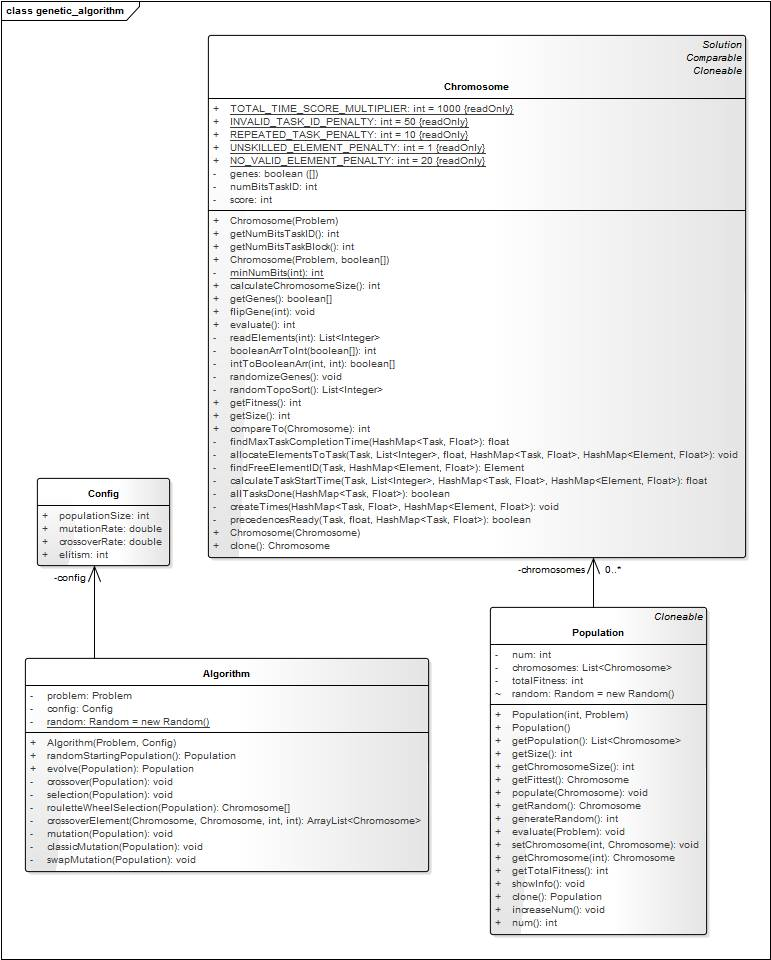
\includegraphics[width=13.5cm, height = 15.5cm]{uml.jpg}
  \caption{Diagrama de classes UML do package \texttt{optimizer.solver.genetic\_algorithm}.}
  \label{uml}
\end{figure}

O projeto foi dividido em packages de forma hierárquica para representar os níveis da solução implementada. Um dos packages serve o propósito de guardar a informação relativa aos membros, tarefas e competências. Outro engloba dois outros packages onde está implementada a solução usando cada um dos algoritmos. O package .gui contém todas as classes que permitem a visualização gráfica da solução encontrada. Esta arquitetura de subpackages foi escolhida por forma a melhor representar a dimensão do problema e da implementação. Na realidade, a hierarquia é o que melhor representa a ligação entre os packages e as suas classes. Esta relação pode ser visualizada na figura \ref{packageD}.

\begin{figure}[H]
  \centering
    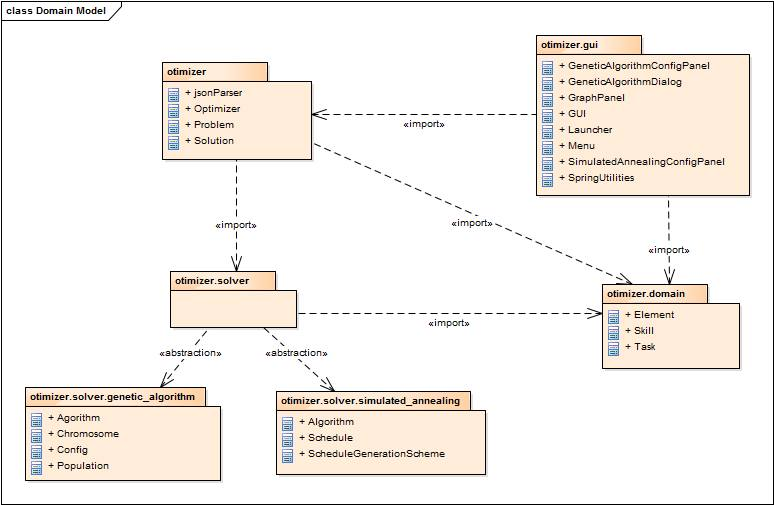
\includegraphics[width=18cm, height = 14cm]{packageDiagram.jpg}
  \caption{Diagrama de packages UML}
  \label{packageD}
\end{figure}

\section{Experiências}

INSERIR EXPERIÊNCIAS AQUI

\section{Conclusões}
\justify\normalsize

INSERIR CONCLUSÕES AQUI

\section{Melhoramentos}
\justify\normalsize

NÃO HÁ MELHORAMENTOS PORQUE ESTÁ DO CRLHHHHHHHH

\nocite{*}
\bibliography{title_page_1}
\bibliographystyle{plain}

\end{titlepage}
\end{document}